
\label{sec:z3}

Celem zadania trzeciego było wykonanie wszechstronnej wizualizacji i interpretacji wyników działania sieci głębokich (oraz klasyfikatorów wykorzystujących ich cechy). W~szczególności zrealizowano następujące etapy:
\begin{enumerate}
    \item \textbf{Analiza błędnych klasyfikacji (misclassifications)} -- identyfikacja i omówienie przypadków, w których model się myli, oraz wskazanie możliwych przyczyn błędów.
    \item \textbf{Wizualizacja obszarów uwagi (CAM, Class Activation Map)} -- sprawdzenie, które fragmenty obrazu mają największy wpływ na odpowiedź modelu.
    \item \textbf{Wizualizacja wewnętrznych warstw (DeepDream)} -- zbadanie i ukazanie sposobu, w jaki wytrenowane filtry sieci reagują na specyficzne wzorce w danych.
    \item \textbf{Testy z własnym zbiorem danych} -- ocena jakości klasyfikatorów na nowym, niestandardowym zbiorze (również generowanym za pomocą \textbf{fooocus v2.5.0} i \emph{Midjourney}) oraz prezentacja metryk (Loss, Accuracy, Top-1 Accuracy, macierze pomyłek, raporty klasyfikacji).
\end{enumerate}

\subsection{Analiza błędnych klasyfikacji}
W~pierwszym kroku dokonano predykcji klas dla wszystkich próbek z~oryginalnego zbioru testowego (zadania 1 i~2), po czym porównano je z rzeczywistymi etykietami. Obrazy sklasyfikowane błędnie zapisywano do osobnego katalogu w celu ich pogłębionej inspekcji (\texttt{misclassified\_images.zip}). 
Przykładowe błędnie sklasyfikowane obrazy dla wersji sieci z klasyfikatorem SVM - jądro poly wraz z etykietami:
\begin{figure}[H]
    \centering
    % Tu wstawić ścieżkę do przykładowego błędnie sklasyfikowanego obrazu
    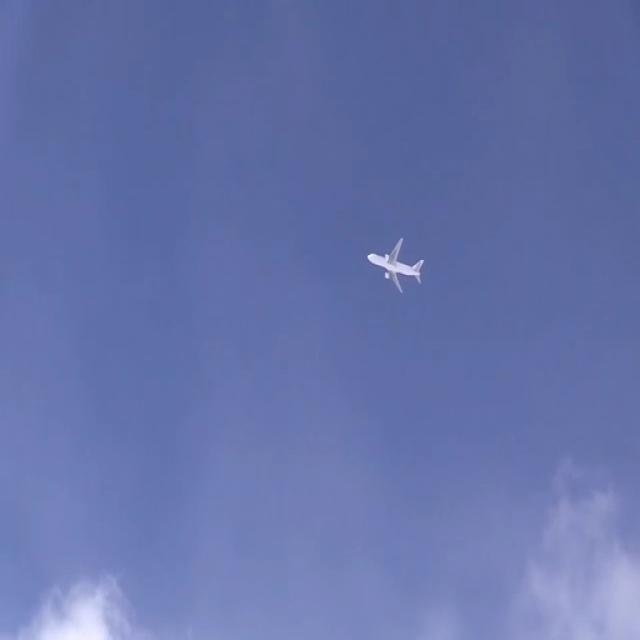
\includegraphics[width=0.55\textwidth]{img/zad3/8_true_samolot_pred_helikopter.png}
    \caption{true - samolot (0), predicted - helikopter (2)}
    \label{fig:z3_misclass}
\end{figure}
\begin{figure}[H]
    \centering
    % Tu wstawić ścieżkę do przykładowego błędnie sklasyfikowanego obrazu
    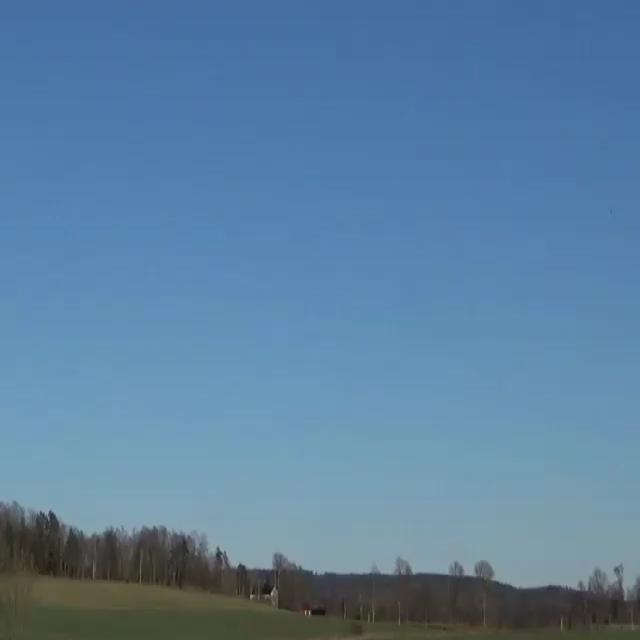
\includegraphics[width=0.55\textwidth]{img/zad3/13_true_ptak_pred_dron.png}
    \caption{true - ptak (3), predicted - dron (1)}
    \label{fig:z3_misclass}
\end{figure}

Najczęstsze przyczyny błędów klasyfikacji to:
\begin{itemize}
    \item \textbf{Niska jakość obrazu:} rozmyte lub nieostre zdjęcia, trudne do zinterpretowania nawet przez człowieka,
    \item \textbf{Podobieństwo klas:} daleki dron przypominający ptaka, nietypowy kształt helikoptera z zewnątrz wyglądający jak samolot,
    \item \textbf{Błędy etykiet (label noise):} istniejące w zbiorze przykłady mogą być niepoprawnie oznakowane,
    \item \textbf{Kontekst otoczenia:} sieć bywała zwodzona np.\ przez specyficzne tło (np.\ chmury, budynki).
\end{itemize}


\subsection{Wizualizacja obszarów uwagi (CAM)}
Aby określić, na które regiony obrazu sieć zwraca największą uwagę, wykorzystano technikę \emph{Class Activation Map (CAM)}:
\begin{itemize}
    \item Z~modelu wybrano ostatnią warstwę splotową (\ \texttt{top\_conv} w \emph{EfficientNetB0}),
    \item Wyliczono gradienty od wyniku klasyfikacji do tejże warstwy, a następnie uśredniono (tzw.\ \emph{global average pooling}),
    \item Otrzymaną mapę \emph{heatmap} nałożono na oryginalny obraz (także w wersji zeskalowanej do~128\texttimes128).
\end{itemize}

Dla wytrenowanych wersji sieci z zadania 1,2a,2b,2c wykonano wizualizację obszarów uwagi dla wybranego obrazu testowego (nr 521). Przykładowe wyniki przedstawiono poniżej:

\begin{figure}[H]
    \centering
    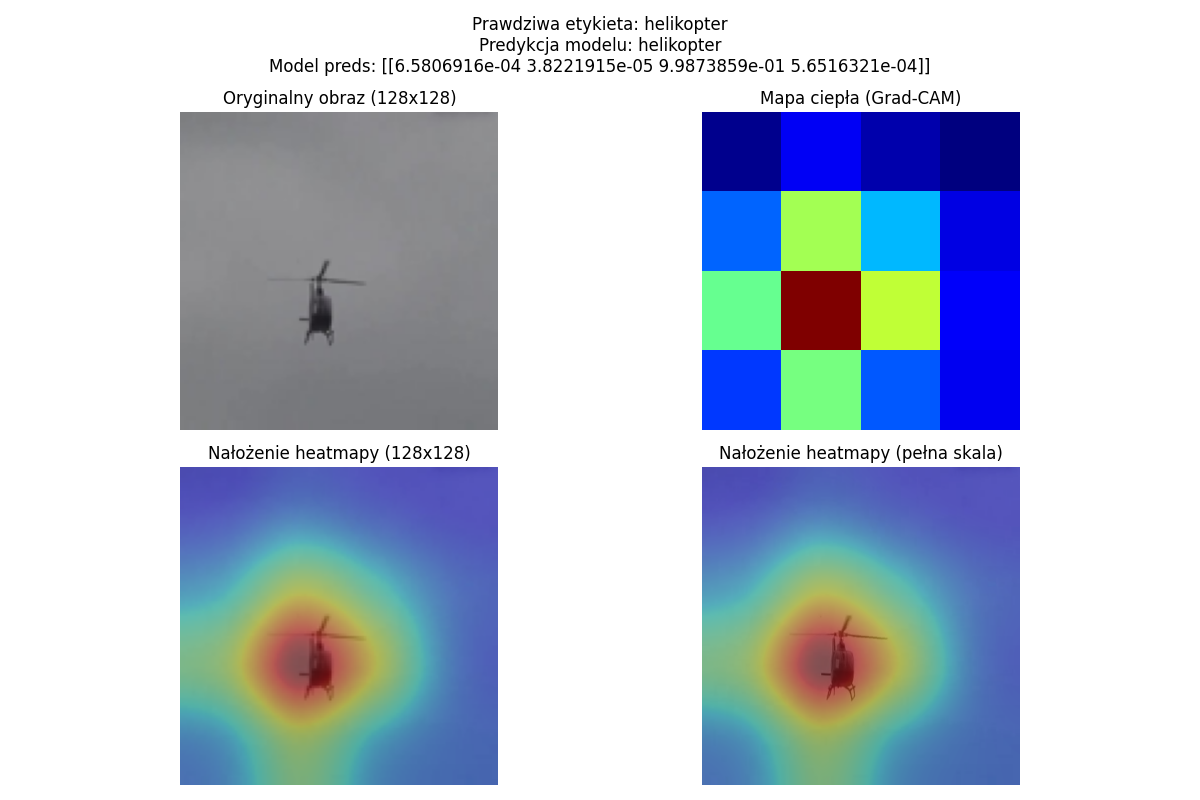
\includegraphics[width=0.9\textwidth]{img/zad3/modelzad1_heatmap_521_true_helikopter_pred_helikopter.png}
    \caption{Przykładowy wynik CAM. Obraz testowy nr. 521 - model z zadania 1 (bez SVM).}
    \label{fig:z3_cam}
\end{figure}
\begin{figure}[H]
    \centering
    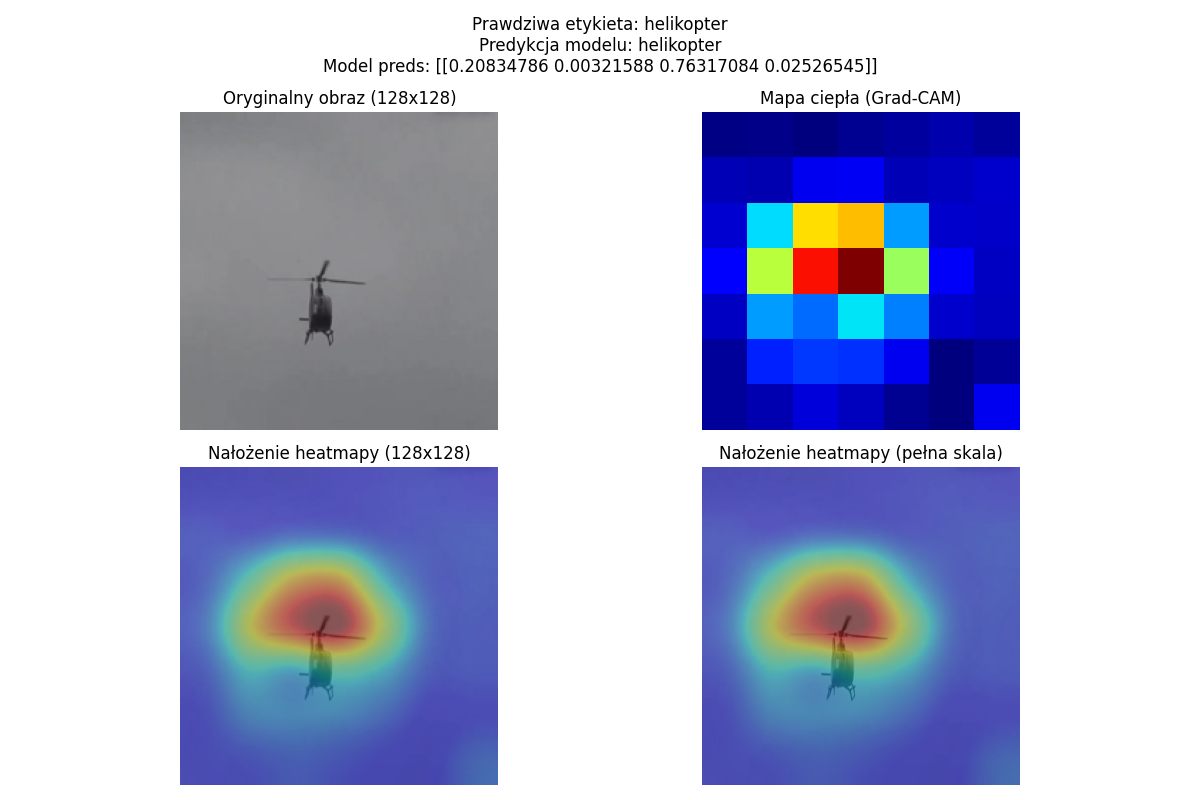
\includegraphics[width=0.9\textwidth]{img/zad3/modelzad2aheatmap_521_true_helikopter_pred_helikopter.png}
    \caption{Przykładowy wynik CAM. Obraz testowy nr. 521 - model z zadania 2a.}
    \label{fig:z3_cam}
\end{figure}
\begin{figure}[H]
    \centering
    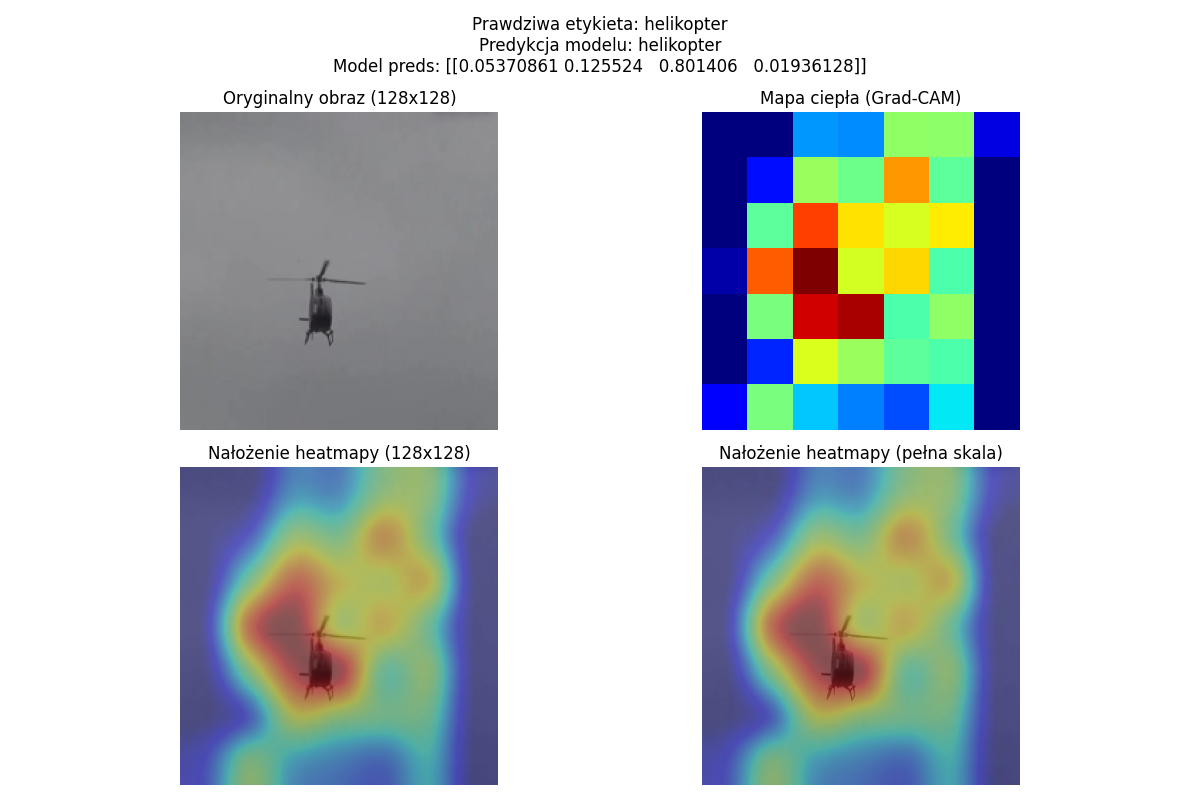
\includegraphics[width=0.9\textwidth]{img/zad3/modelzad2b_heatmap_521_true_helikopter_pred_helikopter.png}
    \caption{Przykładowy wynik CAM. Obraz testowy nr. 521 - model z zadania 2b.}
    \label{fig:z3_cam}
\end{figure}
\begin{figure}[H]
    \centering
    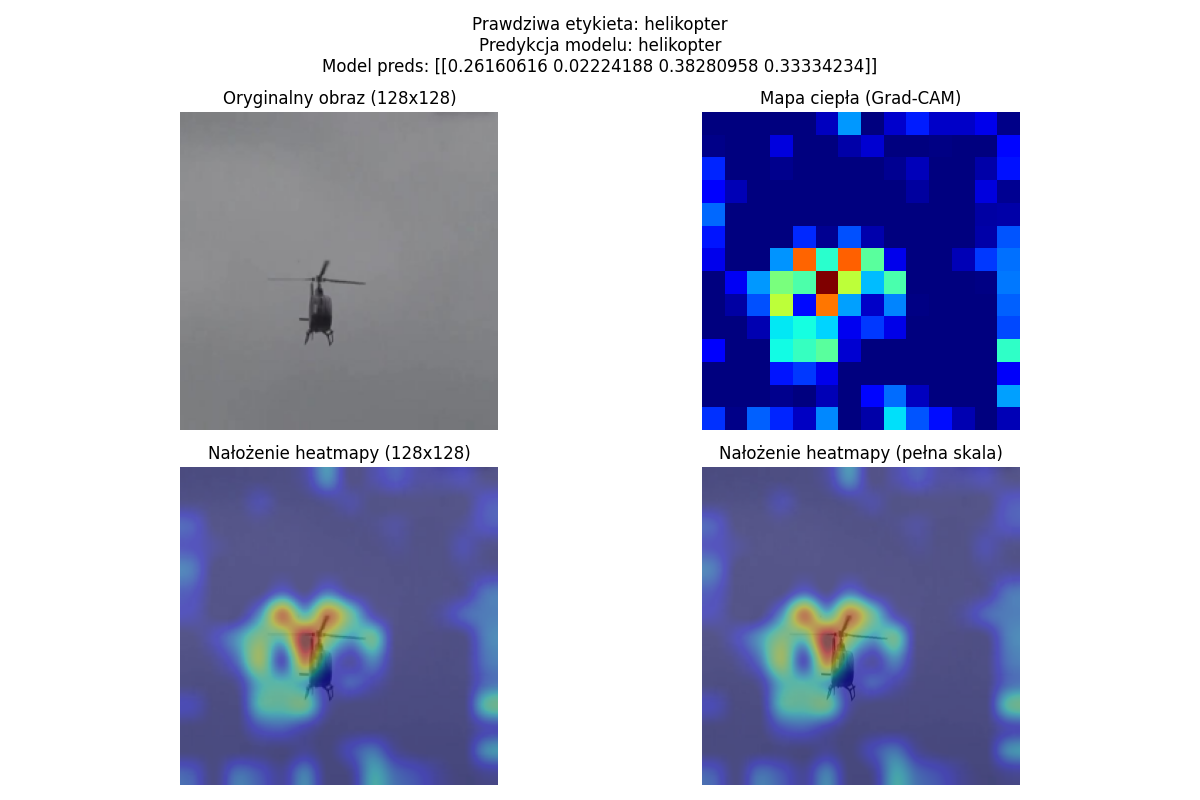
\includegraphics[width=0.9\textwidth]{img/zad3/modelzad2c_heatmap_521_true_helikopter_pred_helikopter.png}
    \caption{Przykładowy wynik CAM. Obraz testowy nr. 521 - model z zadania 2c.}
    \label{fig:z3_cam}
\end{figure}
W prawidłowych klasyfikacjach sieć zwykle koncentruje się na obiekcie (np.\ dronie), natomiast w przypadku błędnych etykiet skupienie może paść na elementy tła i doprowadzić do mylnej decyzji.


\subsection{Wizualizacja wewnętrznych warstw (DeepDream)}
Technika \textbf{DeepDream} umożliwia wizualną eksplorację aktywacji głębszych warstw splotowych:
\begin{itemize}
    \item Dla wybranych warstw (np.\ \texttt{block3a\_activation}, \texttt{block5a\_activation} i \texttt{block7a\_activation} w~\emph{EfficientNetB0}) wykonuje się \emph{gradient ascent} wzmacniający odpowiadające im filtry,
    \item Proces dzieli się na tzw.\ \emph{octave scales}, by uwypuklić różne poziomy szczegółowości (skalowanie w górę obrazu w kolejnych krokach).
\end{itemize}

Wybrany obraz w wersji oryginalnej i po zastosowaniu DeepDream przedstawiono poniżej:
\begin{figure}[H]
    \centering
    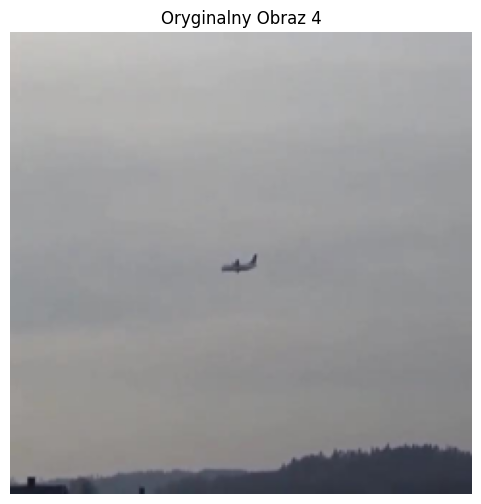
\includegraphics[width=0.6\textwidth]{img/zad3/original4.png}
    \caption{Obraz nr. 4 oryginalny}
    \label{fig:z3_deepdream}
\end{figure}
\begin{figure}[H]
    \centering
    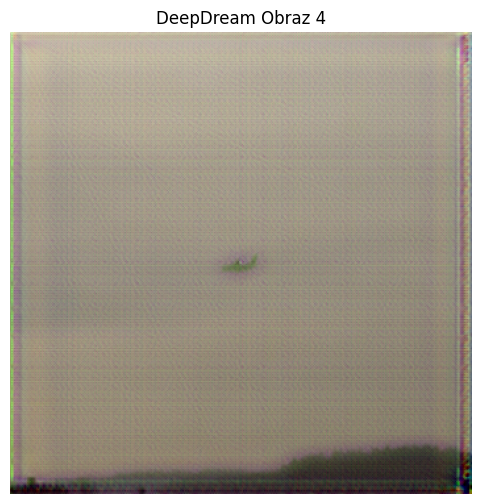
\includegraphics[width=0.6\textwidth]{img/zad3/deepdream4.png}
    \caption{Obraz nr. 4 po zastosowaniu DeepDream (użyto wybranych warstw \emph{EfficientNetB0}).}
    \label{fig:z3_deepdream}
\end{figure}


Jak widać na Rys.~\ref{fig:z3_deepdream}, sieć „uwydatnia” w obrazie wzory przypominające fraktale i abstrakcyjne tekstury, ujawniając tym samym swoje wewnętrzne detektory krawędzi i wzorców.


\subsection{Testy z własnym zbiorem danych i szczegółowe wyniki}
Aby zbadać uogólnianie modeli na dane odbiegające od oryginalnego podziału \texttt{train/valid/test}, wygenerowano \textbf{160 obrazów} (po~40 dla każdej kategorii: \textit{samolot}, \textit{dron}, \textit{helikopter}, \textit{ptak}) za pomocą programu \textbf{Fooocus v2.5.0}, działającego lokalnie na NVIDIA GeForce GTX\,1070.
Przykładowe obrazy z tego zbioru przedstawiono poniżej:

\begin{figure}[H]
    \centering
    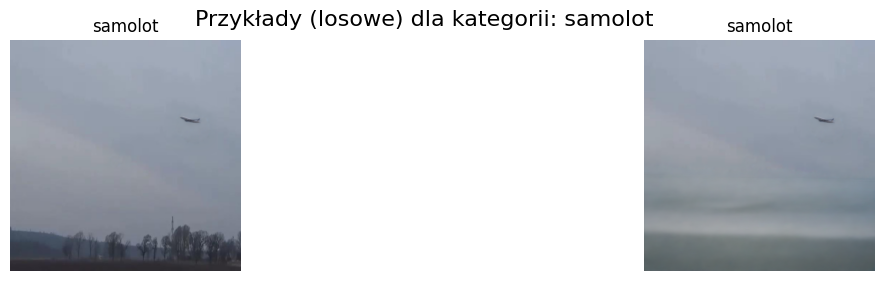
\includegraphics[width=0.95\textwidth]{img/zad3/podpunkt1.png}
    % \caption{Przykładowe obrazy z własnego zbioru danych - kategoria samolot.}
    \label{fig:z3_images}
\end{figure}
\begin{figure}[H]
    \centering
    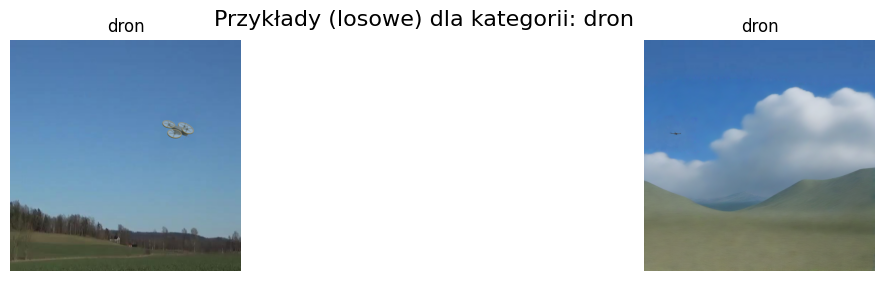
\includegraphics[width=0.95\textwidth]{img/zad3/podpunkt2.png}
    % \caption{Przykładowe obrazy z własnego zbioru danych - kategoria dron.}
    \label{fig:z3_images}
\end{figure}
\begin{figure}[H]
    \centering
    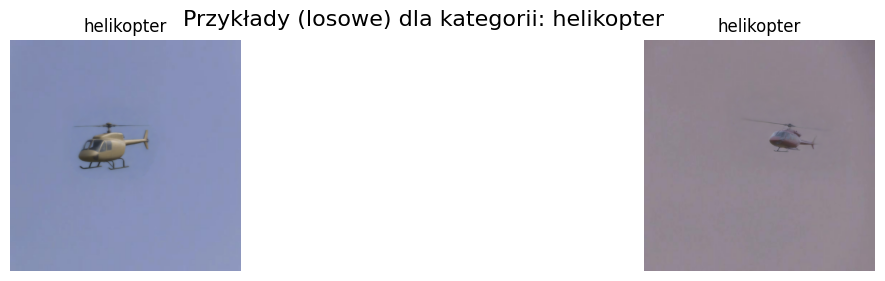
\includegraphics[width=0.95\textwidth]{img/zad3/podpunkt3.png}
    % \caption{Przykładowe obrazy z własnego zbioru danych - kategoria helikopter.}
    \label{fig:z3_images}
\end{figure}
\begin{figure}[H]
    \centering
    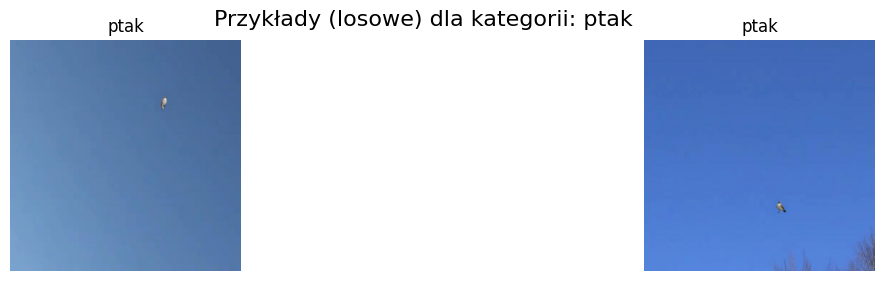
\includegraphics[width=0.95\textwidth]{img/zad3/podpunkt4.png}
    % \caption{Przykładowe obrazy z własnego zbioru danych - kategoria ptak.}
    \label{fig:z3_images}
\end{figure}




Przetestowano cztery finalne modele (z~zadań 1 i 2). Poniżej przedstawiono zestawienia uzyskanych metryk, macierzy pomyłek i raportów klasyfikacji.

\subsubsection*{Model \texttt{umir\_model\_zad1.keras}}
\begin{itemize}
    \item \textbf{Loss:} 4.3591 \quad \textbf{Accuracy:} 0.3125 \quad \textbf{Top-1 Accuracy:} 0.3125
\end{itemize}

\begin{table}[H]
\centering
\caption{Macierz pomyłek (\texttt{umir\_model\_zad1}) na zbiorze 160 obrazów.}
\begin{tabular}{c|cccc}
\hline
 & \textbf{samolot} & \textbf{dron} & \textbf{helikopter} & \textbf{ptak} \\ 
\hline
\textbf{samolot}     & 0 & 0 & 40 & 0 \\
\textbf{dron}        & 1 & 10 & 29 & 0 \\
\textbf{helikopter}  & 0 & 0 & 40 & 0 \\
\textbf{ptak}        & 0 & 0 & 40 & 0 \\
\hline
\end{tabular}
\end{table}

\noindent


\subsubsection*{Model \texttt{umir\_model\_zad2a.keras}}
\begin{itemize}
    \item \textbf{Loss:} 1.5077 \quad \textbf{Accuracy:} 0.3938 \quad \textbf{Top-1 Accuracy:} 0.3937
\end{itemize}

\begin{table}[H]
\centering
\caption{Macierz pomyłek (\texttt{umir\_model\_zad2a}) na zbiorze 160 obrazów.}
\begin{tabular}{c|cccc}
\hline
 & \textbf{samolot} & \textbf{dron} & \textbf{helikopter} & \textbf{ptak}\\
\hline
\textbf{samolot}     & 20 &  0 & 20 &  0 \\
\textbf{dron}        & 17 &  5 & 18 &  0 \\
\textbf{helikopter}  &  2 &  0 & 38 &  0 \\
\textbf{ptak}        &  0 &  0 & 40 &  0 \\
\hline
\end{tabular}
\end{table}

\noindent



\subsubsection*{Model \texttt{umir\_model\_zad2b.keras}}
\begin{itemize}
    \item \textbf{Loss:} 2.4320 \quad \textbf{Accuracy:} 0.2250 \quad \textbf{Top-1 Accuracy:} 0.2250
\end{itemize}

\begin{table}[H]
\centering
\caption{Macierz pomyłek (\texttt{umir\_model\_zad2b}) na zbiorze 160 obrazów.}
\begin{tabular}{c|cccc}
\hline
 & \textbf{samolot} & \textbf{dron} & \textbf{helikopter} & \textbf{ptak}\\
\hline
\textbf{samolot}     & 0 &  0 & 40 &  0 \\
\textbf{dron}        & 0 &  2 & 38 &  0 \\
\textbf{helikopter}  & 0 &  6 & 34 &  0 \\
\textbf{ptak}        & 0 &  0 & 40 &  0 \\
\hline
\end{tabular}
\end{table}

\noindent


\subsubsection*{Model \texttt{umir\_model\_zad2c.keras}}
\begin{itemize}
    \item \textbf{Loss:} 1.3587 \quad \textbf{Accuracy:} 0.3750 \quad \textbf{Top-1 Accuracy:} 0.3750
\end{itemize}

\begin{table}[H]
\centering
\caption{Macierz pomyłek (\texttt{umir\_model\_zad2c}) na zbiorze 160 obrazów.}
\begin{tabular}{c|cccc}
\hline
 & \textbf{samolot} & \textbf{dron} & \textbf{helikopter} & \textbf{ptak}\\
\hline
\textbf{samolot}     &  1 & 24 & 13 &  2 \\
\textbf{dron}        & 17 & 19 &  3 &  1 \\
\textbf{helikopter}  &  0 &  0 & 40 &  0 \\
\textbf{ptak}        &  0 &  0 & 40 &  0 \\
\hline
\end{tabular}
\end{table}

\noindent

\subsection{Wnioski z zadania 3}

\begin{itemize}
    \item \textbf{Analiza błędnych klasyfikacji} (Rys.~\ref{fig:z3_misclass}) pomogła wyodrębnić najtrudniejsze przypadki (mała rozdzielczość, nietypowe kąty, stylizowane obrazy). 
    \item \textbf{Wizualizacje CAM} (Rys.~\ref{fig:z3_cam}) potwierdziły, że poprawne predykcje wynikają najczęściej z właściwego ukierunkowania uwagi na docelowy obiekt (kadłub samolotu, drona, helikoptera). W~przypadku błędów model często skupia się na elementach tła.
    \item \textbf{DeepDream} (Rys.~\ref{fig:z3_deepdream}) odsłonił charakterystyczne wzorce detektorów (np.\ krawędzi, faktur), które sieć „wzmacnia” w trakcie procesu \emph{gradient ascent}.
    \item \textbf{Eksperyment z własnym zbiorem danych}, który uwzględniał \textbf{160 obrazów} z programu \textbf{Fooocus v2.5.0} (po~40 na klasę), pokazał słabości modeli w kontekście wysoce nietypowych, generowanych ujęć. 
    \begin{itemize}
        \item \texttt{umir\_model\_zad1} i \texttt{umir\_model\_zad2b} wypadły najsłabiej (w tym konkretnym eksperymencie) pod względem \emph{Accuracy} (0.31 i 0.23), co wskazuje na potencjalną nieadekwatność treningu do tak różnorodnego stylu obrazów,
        \item \texttt{umir\_model\_zad2a} i \texttt{umir\_model\_zad2c} osiągnęły nieco wyższe wyniki (ok.\ 0.39 i 0.38), choć ogólny poziom jest wciąż daleki od zadowalającego,
        \item modele miewały szczególne problemy w rozróżnianiu \emph{ptaków} i \emph{dronów} w stylizowanych scenach — \emph{recall} i \emph{precision} dla tych klas były często niskie.
    \end{itemize}
\end{itemize}

\noindent
Wyniki te pokazują, że większe zróżnicowanie (i~szersze dostrojenie) bazy treningowej lub bardziej rozbudowane sieci mogłyby poprawić sprawność klasyfikacji na \emph{generowanych} (nietypowych) obrazach. 
